\documentclass{standalone}

\begin{document}
	It is now time to evaluate our implemented application by performing a critical analysis to help determine the extent of our application's fulfilment to the initial project goals. This shall be done by performing a series of both objective and subjective tests aiming to expose its strengths and weaknesses. All experiments are performed on machine with an Intel Core i7 3770K CPU (3.5 GHz) and 16GB RAM (1600 Mhz).

	\begin{figure}[!htbp]
		\centering
		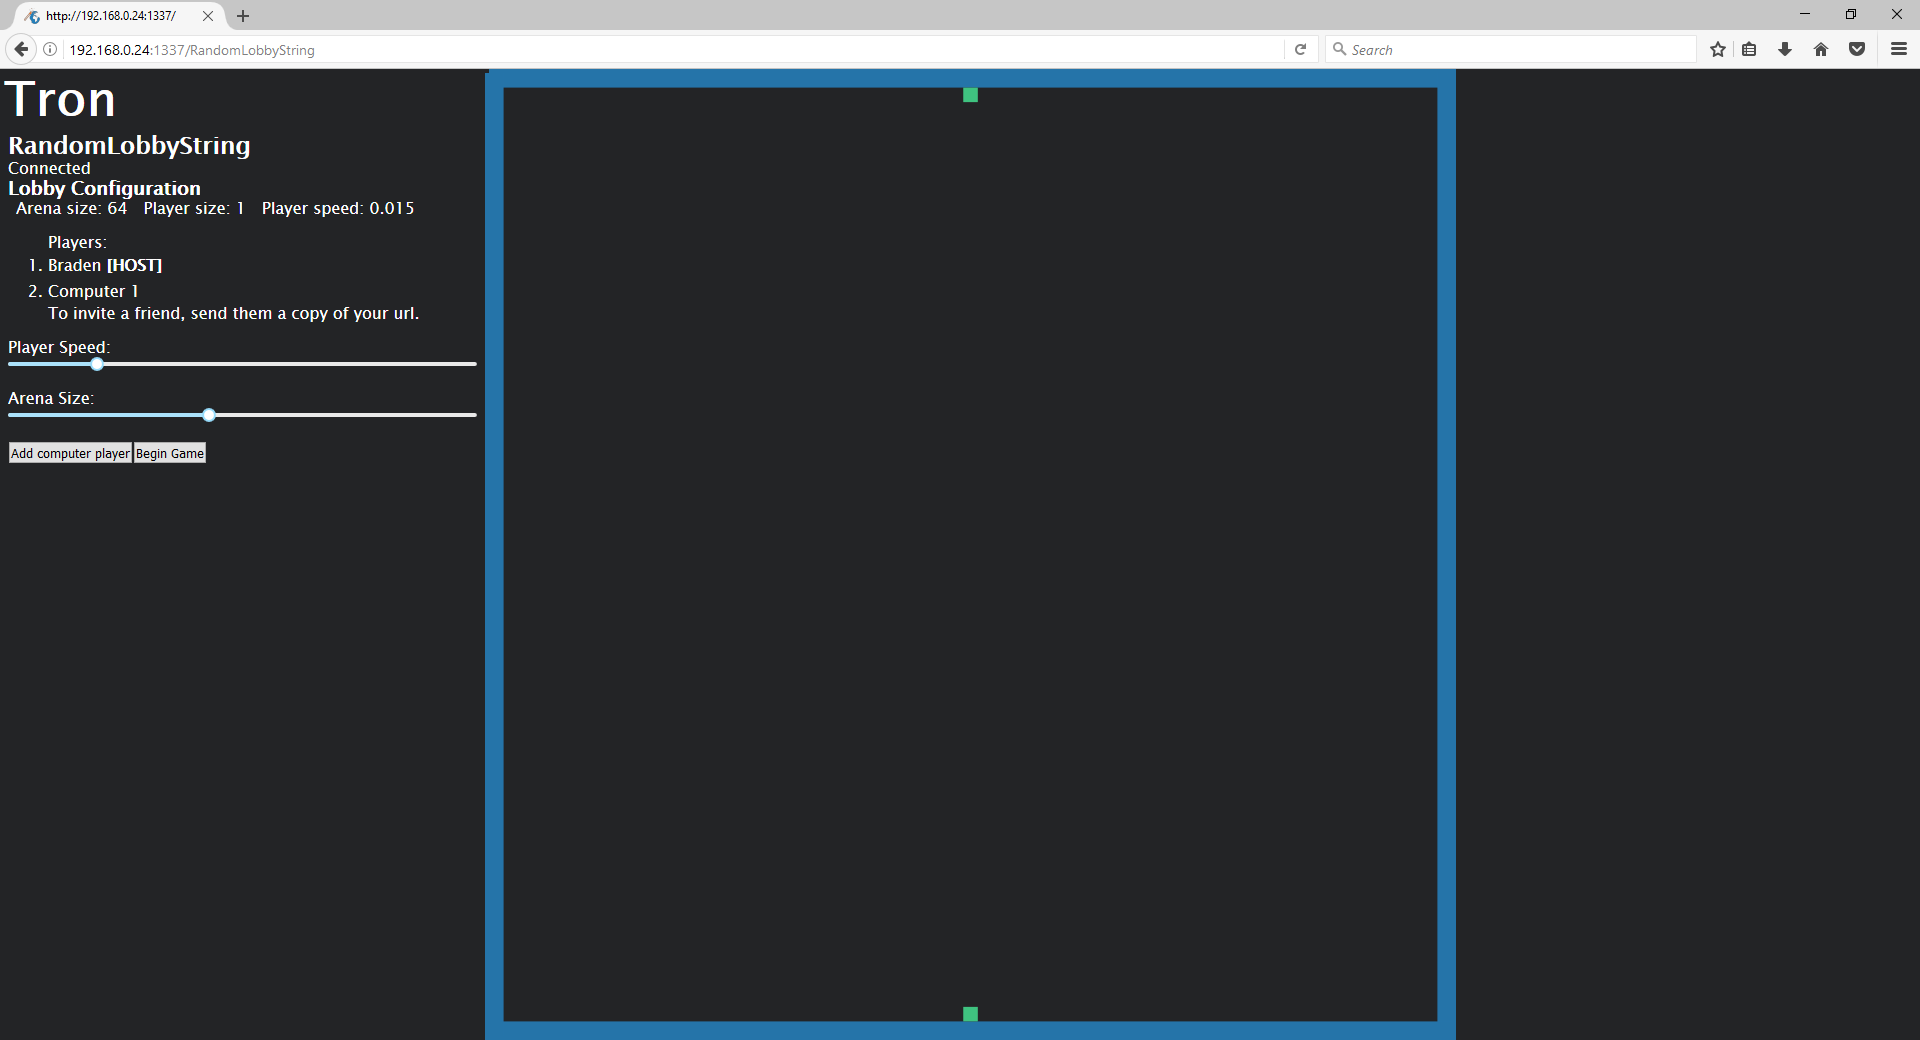
\includegraphics[width=\textwidth]{resources/images/inbrowser.png}
		\caption{Screen capture of the implemented application, demonstrating the game within a web-browser.}
	\end{figure}
	\FloatBarrier

	\begin{figure}[!htbp]
		\centering
		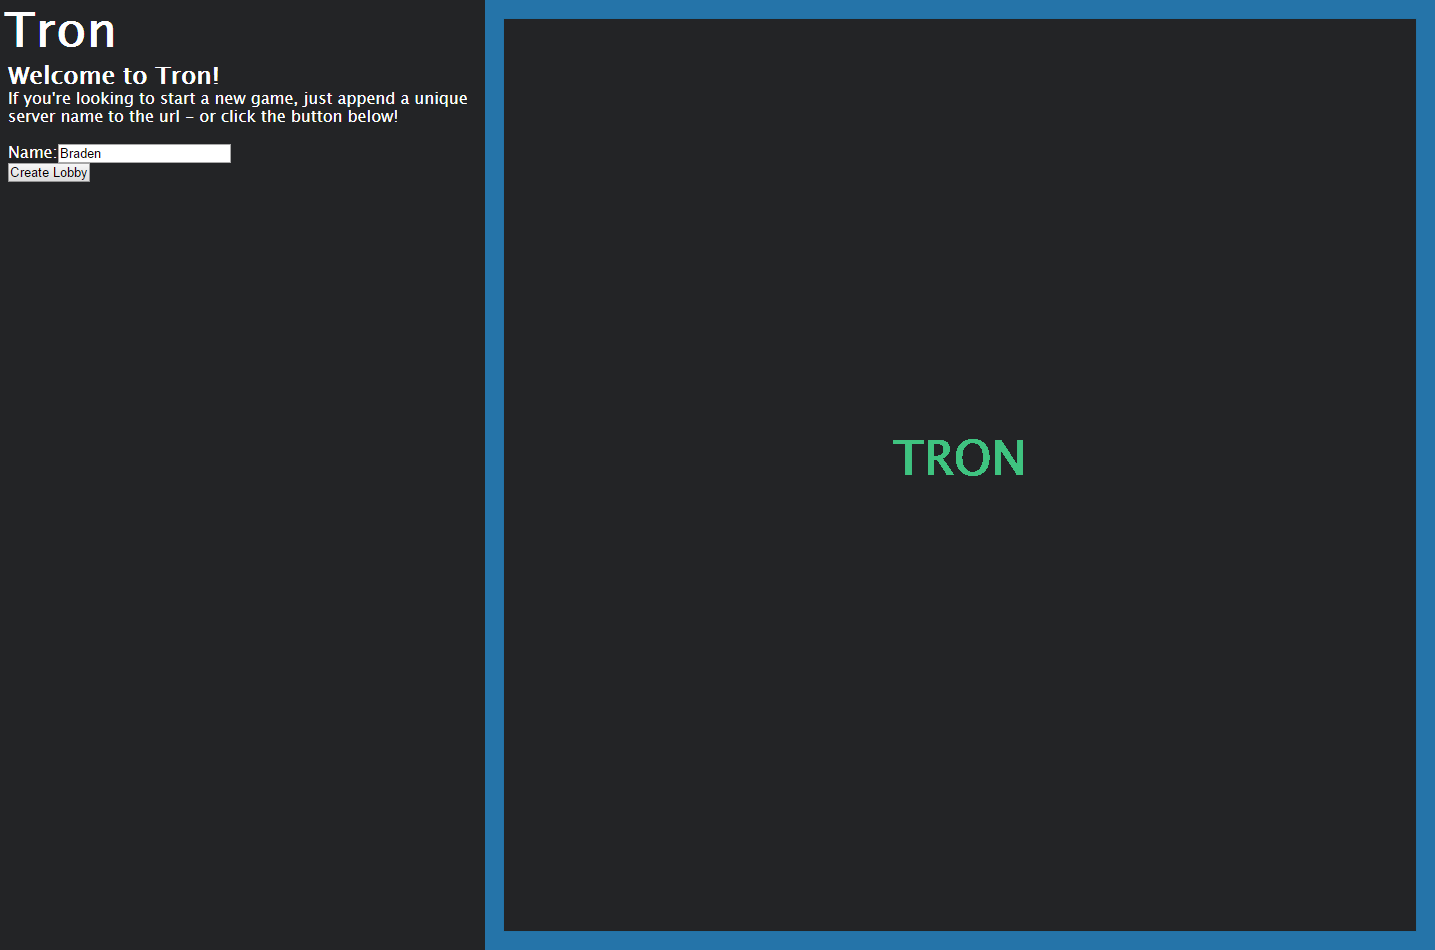
\includegraphics[width=\textwidth]{resources/images/welcome.png}
		\caption{Screen capture of the implemented application, demonstrating the game's welcome screen.}
	\end{figure}
	\FloatBarrier

	\begin{figure}[!htbp]
		\centering
		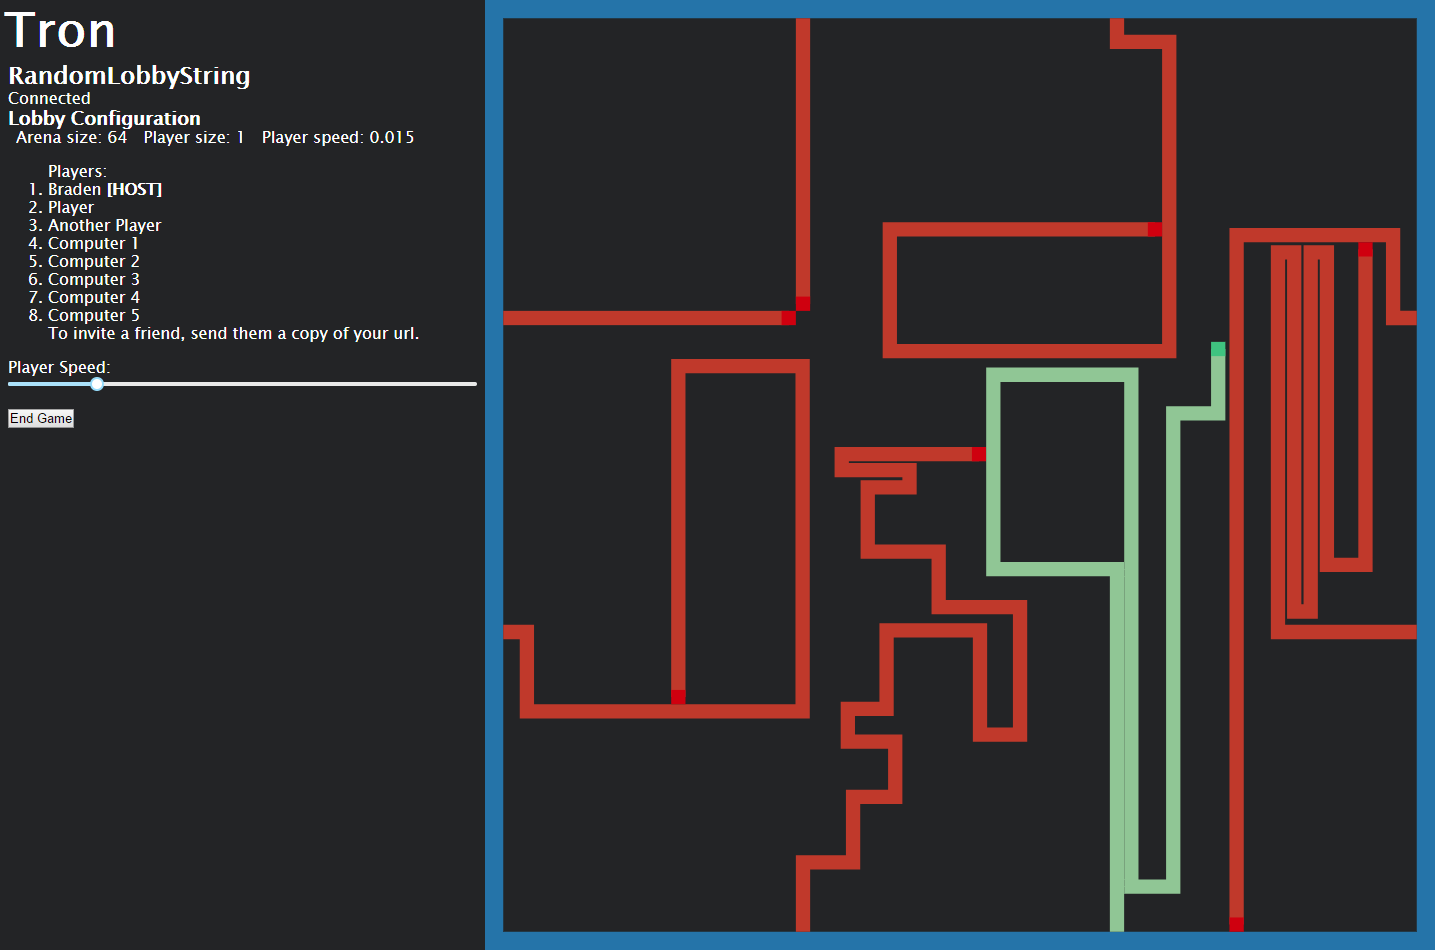
\includegraphics[width=\textwidth]{resources/images/ingame.png}
		\caption{Screen capture of the implemented application, demonstrating the game in progress.}
	\end{figure}
	\FloatBarrier

	\section{Unit Tests}
		Unit testing is arguably the most reliable software development technique for the purposes of scrutinizing an application in order to prove its operational correctness. A unit is the smallest testable part of an application, such as an individual function. A unit test is a short code fragment intended to test a single unit of an application.

		During the development process, an application will evolve as modifications are introduced. This is normal behaviour, although the process has a habit of leaving behind bugs. Having a complete suite of unit tests enable the developer to automatically identify bugs and ensure that their code retains its previous validity. Unit tests can be implemented in a number of ways. As the meat of our application is programmed in JavaScript, we will be using Jest \parencite{jest} - one of the many available JavaScript testing solutions. Jest also offers specialised support for React via snapshot testing. Various modules within our application contain unit tests in a subdirectory named \enquote{\texttt{\_\_tests\_\_}}. These tests have been developed according to both the black-box and white-box testing methods, to best guarantee the completeness of our application.\footnote{Due to the time-sensitive nature of the project, the currently implemented unit tests do not yet have 100\% coverage of our application.}

		\begin{figure}[!htbp]
			\begin{formal}
				\verbatiminput{unittestoutput.tex}
			\end{formal}
			\caption{Capture of the console output produced from executing our Jest unit tests.} \label{fig:unitTests}
		\end{figure}

		As seen from \autoref{fig:unitTests}, we have unit tests covering several modules of our application. Should a new bug be discovered within one of these modules, a new test would be created capable of detecting said bug. For information regarding what is actually being tested, we encourage the reader to refer to the JavaScript test file's source-code; they are well documented.

	\section{Game Performance}
		The game has been developed up to a playable state, yet there is still interest in seeing just how much is capable before it begins to breakdown. To gain a stronger understanding of just what our game is capable of, we conduct experiments measuring the performance impact caused by various game mechanics. For each of these experiments, the goal is to derive a sensible evaluation based upon an accumulation of quantifiable data.\footnote{A separate Git branch was created for the purposes of recording benchmark data. It can be found on our GitHub repository (see \fullref{sec:softwareDevelopmentProcess}).}

		\subsection{Tick Update Performance} \label{sec:tickUpdatePerformance}
			The game loop is responsible for drawing the graphics and, more importantly, updating the game state. It is absolutely critical that the update function's call duration does not exceed the duration of its associated tick. If this were the case, our game's tick-rate would begin to fall - leading to undesired game behaviour. Hence we perform a series of experiments measuring the implemented update function's execution duration under various scenarios. These scenarios will vary by two controllable factors: the total number of connected players\footnote{All connected players, besides the host player, are computer players controlled by artificial intelligence. This means our results better resemble those of worst-case performance.}, and the elapsed time since the beginning of the game round. Each experiment scenario is repeated five times to help mitigate erroneous results.\footnote{For a full log detailing the exact results gathered from the experiment, refer to \autoandpageref{tab:gamePerformance}.}

			\subimport{resources/performance/}{graph.tex}

			As can be seen in \autoref{fig:gamePerformanceChart}, the results indicate there is definitely a significant correlation between our game's performance and the two examined factors. It can be seen that an increase to either factor will result in our game state update duration being prolonged. Not only this, but performance is subject to the combination of either factor. The reasoning for this is quite simple, and our collision detection is the primary cause: in general, our collision detection is required to perform more extensive searches if our game arena consists of a greater number of objects. Furthermore, as the round naturally progresses in time, each player will be travelling around the game arena; contributing additional objects. Hence, round progression produces objects proportionally to the number of alive players; further burdening the task of collision detection. However with this being said, even in the worst case, our game state updates occur at an extremely fast rate - well within the required bounds of once every 15 milliseconds (see \fullref{sec:gameMechanics}).

	\section{Capability of Artificial Intelligence} \label{sec:aiCapabilities}
		Each computer player determines their move using an artificial intelligence, powered by the culmination of various techniques. The goal of which is to mimic the behaviour of a human controlled player, giving the competing human user(s) a realistic game experience. This happens to be quite a difficult requirement to test, due to the subjectiveness of what can be considered \enquote{human behaviour} (for a relevant subjective experiment, see \autoref{sec:userFeedback}). Despite this, we can obtain empirically quantifiable data by running a series of experiments, recording the win-percentage gathered from pitching our implemented AI against a human controlled player. Ideally, we would like the AI player to perform equally to the human user, i.e. a 50/50 win-ratio. However, the results are subject to the skill-level of the competing human user. This is not something that we can easily regulate, so we assume our chosen human user is of an average skill-level. To get a broad understanding, we shall be performing the experiment under several different scenarios, varying the game by certain factors. These factors include the game arena size and player movement speed. We shall capture the total simulation count at the start of each round, then select the median result from five repeats to help mitigate erroneous results.

		\subimport{resources/ai/}{capabilitytable.tex}

		As can be seen in \autoref{tab:aiWins}, the computer player performs somewhat respectably in comparison to a human user. From observing the experiments, the artificial intelligence would often begin with reasonable strategy, but then occasionally decide to play a move that was not so favourable. This was especially a problem in the larger arena sizes, once the two competing players had become disconnected from one-another. Once the two players would separate, the human controlled player was able to simply wait for the computer player to make a mistake. Hence, the AI performed particularly well when the arena size was smaller, due to the generally shorter game duration. The computer player thrived at faster speeds, as the human player was unable to react expeditiously. However, a combination of the tested fastest speed and smallest arena size, made the game feel somewhat random - as both players were unable to make strategic moves. To better understand where improvements could be made, analysis was performed regarding the performance of our simulations. This prompted investigation into how the total simulation count was affected by the size of the game arena.

		\subimport{resources/ai/}{simulationgraph.tex}
		\FloatBarrier

	 	As expected (see \autoref{fig:aiSimulationCount})\footnote{For a full log detailing the exact results gathered from the simulation count experiment, refer to \autoandpageref{tab:aiSimulationCount}.}, the total simulation count is considerably greater for arenas of a relatively smaller size. This indicates something within our simulation task was hindering performance. However, expanding from what was shown in \fullref{sec:tickUpdatePerformance}, it was suspected that game update function was not to blame, but instead the heuristic evaluation function. This suspicion was proven correct by dramatically increasing the simulation depth and measuring how it affected the total number of simulations (see \autoref{fig:aiSimulationDepth})\footnote{For a full log detailing the exact results gathered from the simulation depth experiment, refer to \autoandpageref{tab:aiSimulationDepth}.}. This experiment will be performed with two players, one controlled by a human and the other by our artificial intelligence. We shall record the median value of five initial computer moves, made on an arena size of 32. If the total number of simulations sparsely changed, we would know that our heuristic evaluation function was to blame; as it ran only at the end of a simulation - unaffected by depth. This loss of performance would prevent the proper construction of belief regarding the game tree, leading to the move being decided upon despite not having fully explored the consequences.

		\subimport{resources/ai/}{simulationdepthgraph.tex}
		\FloatBarrier

		Another fault of our artificial intelligence is regarding timing. The simulation tree would often try to play optimally, for example by redirecting at the very last instant. This is caused by the simulation believing it has control over the next move. Sadly, this is not the case due to the non-deterministic nature involved for the concurrent aspects of our application. Despite efforts made to remedy this (see \fullref{sec:aiTiming}), the issue still persists - although not to its previous extent.

		The artificial intelligence also has no explicit means to prevent itself from blocking off \enquote{owned} areas of the game arena. This results in the computer player often making moves that will worsen their total potential lifespan. The issue has been tackled by others (see \fullref{sec:background-google-ai}). but was never included in our implementation.

		As discussed in \fullref{sec:aiConcurrency}, our artificial intelligence calculates moves in a process separate to that running the main application. This functionality works quite well for a game consisting of only several computer players, but begins to fall down when a larger quantity of computer players are introduced. In part, this is due to each computer player being assigned their own process to calculate moves; an architecture which does not scale well, due to the executing computer only have a limited number of cores.

	\section{User Feedback} \label{sec:userFeedback}
		The implemented game could be objectively perfect, however if users believe that the project fails to hold promise, then our project's investigated ambition would conclude as a failure - indicating the designed techniques fail to perform sufficiently. Therefore, it is worthwhile to collect a sample of user opinions, enabling us to form a concrete understanding of where our application stands. Hence, we introduce five users to play a few games, then document their opinions by having them participate in a short survey, as described in \autoref{fig:userSurvey}.

		\begin{figure}[!htbp]
			\begin{formal}
				Please respond to the below questions on a scale from 1-10 (where 1 is strongly disagree, and 10 is strongly agree):
				\begin{enumerate}
					\item The graphics of the game appear to run smoothly.
					\item The game's user interface is functional, with near unnoticeable loading times. 
					\item Movement around the game arena seemed sufficiently accurate, in response to my input.
					\item The multiplayer functionality felt responsive, with little indication of latency.
					\item The computer controller player works well; challenging, but not impossible to beat.
					\item The foundational mechanics of the game hold promise, and could produce a good game with a little more polish.
				\end{enumerate}
				\caption{A series of questions to be surveyed to test participants.} \label{fig:userSurvey}
			\end{formal}
		\end{figure}
		\FloatBarrier

		For the most part, user feedback (see \autoandpageref{tab:userSurveyResults}) indicates that the game is somewhat a success. Although this is pleasing, it fails to highlight the weak-points of our application.
\end{document}